\KOMAoption{paper}{a4, portrait}
\areaset{267mm}{180mm}
\fancyheadoffset{0pt} % обновляем хедер и футер

\newgeometry{
  top=14mm,
  bottom=11mm,
  right=10mm,
  left=22mm,
}

\begin{landscape}

%\setlength{\headsep}{5.6mm} 
%\setlength{\topmargin}{-27mm}
\setlength{\footskip}{15.5pt}
%\setlength{\textwidth}{305mm}

\color{uniblue}{\section[(справочное) Перечень сигналов ФСУ, предназначенных для \newline конфигурирования устройства]{(справочное)\\Перечень сигналов ФСУ, предназначенных для конфигурирования устройства}\label{app:signals}}
\color{black}

\begin{enumerate}[label=\ref{app:signals}.\arabic*] % Без глобального влияния
  \item Перечень сигналов самодиагностики, доступных для конфигурирования, приведен в документации \ManualUnitGeneral.
  \item Условные обозначения, применяемые в таблице перечня сигналов:
  \begin{itemize}
    \item[$\text{(--)}$] { - сигнал не имеет возможности конфигурации;}
    \item[$\text{(+)}$] { - сигнал имеет возможность конфигурации;}
    \item[$\text{(*)}$] { - конфигурация сигнала предустановлена по умолчанию в сервисном ПО «ЮНИТ-СЕРВИС РЗА» и не может быть изменена.}
  \end{itemize}
\end{enumerate}

\small % сделаем шрифт в таблице поменьше
% В таблице ниже убрал правую и левую горизонтальные линии чтобы не сливались и жирно видно - также в настройках geometry прищлось поле right =8mm а не 5 mm 
% так как строки ниже колонтитулов спускались
\begin{longtable}{
>{\centering\arraybackslash}m{6.0cm}
|>{\centering\arraybackslash}m{3.45cm}
|>{\centering\arraybackslash}m{2cm}
|>{\centering\arraybackslash}m{2cm}
|>{\centering\arraybackslash}m{2cm}
|>{\centering\arraybackslash}m{2cm}
|>{\centering\arraybackslash}m{2cm}
|>{\centering\arraybackslash}m{2cm}
|>{\centering\arraybackslash}m{2.107cm}
}

%\caption{Перечень сигналов ФСУ, предназначенных для конфигурирования устройств ЮНИТ-М300\vspace{-0.5\baselineskip}}\label{appA:tbl1}\\ % выравнивает надпись посередине таблицы
\caption{Перечень сигналов ФСУ, предназначенных для конфигурирования устройства\hfill\vspace{-0.5\baselineskip}}\label{appA:tbl1}\\ 

\hline
\rowcolor{gray!30}
Полное наименование сигнала & Наименование сигнала на ФСУ & Дискретные входы & Выходные реле & Светодиоды & Функционал. клавиши & Регистратор событий & Аварийный осциллограф & Пуск авар. осциллографа \\ 
\hline
\endfirsthead
%\caption{\emph{Продолжение\vspace{-0.5\baselineskip}}} \\ % Отступ обозначения таблицы от таблицы и выравнивание надписи слева
\caption*{\hspace{3pt}\emph{Продолжение таблицы \ref{appA:tbl1}\hfill\vspace{-0.5\baselineskip}}} \\ % сделано по ГОСТ 2.105 п.6.8.7
\hline
\rowcolor{gray!30}
Полное наименование сигнала & Наименование сигнала на ФСУ & Дискретные входы & Выходные реле & Светодиоды & Функционал. клавиши & Регистратор событий & Аварийный осциллограф & Пуск авар. осциллографа \\ 
%\hline
\endhead

%\hline
\endfoot

%\hline
\endlastfoot

%===t2
\multicolumn{9}{c}{\textbf{Общие сигналы функциональной логики}} \\
\hline
\rowcolor{gray!15}
\multicolumn{9}{c}{АПВ } \\
\hline
\multicolumn{9}{c}{\text{АПВ Э1}} \\
\hline
\raggedright АПВ/ АПВ Э1: Режим ведомый & \centering АПВ/ АПВ Э1: Режим ведомый & \centering -- & \centering -- & \centering -- & \centering -- & \centering -- & \centering -- & \centering \arraybackslash -- \\ \hline
\raggedright АПВ/ АПВ Э1: Режим без контролей & \centering АПВ/ АПВ Э1: Режим без контролей & \centering -- & \centering -- & \centering -- & \centering -- & \centering -- & \centering -- & \centering \arraybackslash -- \\ \hline
\raggedright АПВ/ АПВ Э1: Нет усл. вкл. & \centering АПВ/ АПВ Э1: Нет усл. вкл. & \centering -- & \centering -- & \centering -- & \centering -- & \centering -- & \centering -- & \centering \arraybackslash -- \\ \hline
\raggedright АПВ/ АПВ Э1: Выведено & \centering АПВ/ АПВ Э1: Выведено & \centering -- & \centering -- & \centering -- & \centering -- & \centering -- & \centering -- & \centering \arraybackslash -- \\ \hline
\raggedright АПВ/ АПВ Э1: Ср. 1ц & \centering АПВ/ АПВ Э1: Ср. 1ц & \centering -- & \centering -- & \centering -- & \centering -- & \centering -- & \centering -- & \centering \arraybackslash -- \\ \hline
\raggedright АПВ/ АПВ Э1: Включить & \centering АПВ/ АПВ Э1: Включить & \centering -- & \centering -- & \centering -- & \centering -- & \centering -- & \centering -- & \centering \arraybackslash -- \\ \hline
\raggedright АПВ/ АПВ Э1: Ср. 2ц & \centering АПВ/ АПВ Э1: Ср. 2ц & \centering -- & \centering -- & \centering -- & \centering -- & \centering -- & \centering -- & \centering \arraybackslash -- \\ \hline
\raggedright АПВ/ АПВ Э1: П. 2ц & \centering АПВ/ АПВ Э1: П. 2ц & \centering -- & \centering -- & \centering -- & \centering -- & \centering -- & \centering -- & \centering \arraybackslash -- \\ \hline
\raggedright АПВ/ АПВ Э1: Пуск & \centering АПВ/ АПВ Э1: Пуск & \centering -- & \centering -- & \centering -- & \centering -- & \centering -- & \centering -- & \centering \arraybackslash -- \\ \hline
\raggedright АПВ/ АПВ Э1: П. 1ц & \centering АПВ/ АПВ Э1: П. 1ц & \centering -- & \centering -- & \centering -- & \centering -- & \centering -- & \centering -- & \centering \arraybackslash -- \\ \hline
\raggedright АПВ/ АПВ Э1: Гот. 2ц & \centering АПВ/ АПВ Э1: Гот. 2ц & \centering -- & \centering -- & \centering -- & \centering -- & \centering -- & \centering -- & \centering \arraybackslash -- \\ \hline
\raggedright АПВ/ АПВ Э1: Готовность & \centering АПВ/ АПВ Э1: Готовность & \centering -- & \centering -- & \centering -- & \centering -- & \centering -- & \centering -- & \centering \arraybackslash -- \\ \hline
\raggedright АПВ/ АПВ Э1: Гот. 1ц & \centering АПВ/ АПВ Э1: Гот. 1ц & \centering -- & \centering -- & \centering -- & \centering -- & \centering -- & \centering -- & \centering \arraybackslash -- \\ \hline
\raggedright АПВ/ АПВ Э1: КЗ отключено & \centering АПВ/ АПВ Э1: КЗ отключено & \centering -- & \centering -- & \centering -- & \centering -- & \centering -- & \centering -- & \centering \arraybackslash -- \\ \hline
\raggedright АПВ/ АПВ Э1: В включен от АПВ & \centering АПВ/ АПВ Э1: В включен от АПВ & \centering -- & \centering -- & \centering -- & \centering -- & \centering -- & \centering -- & \centering \arraybackslash -- \\ \hline
\raggedright АПВ/ АПВ Э1: Успешное АПВ & \centering АПВ/ АПВ Э1: Успешное АПВ & \centering -- & \centering -- & \centering -- & \centering -- & \centering -- & \centering -- & \centering \arraybackslash -- \\ \hline
\raggedright АПВ/ АПВ Э1: Неуспешное АПВ & \centering АПВ/ АПВ Э1: Неуспешное АПВ & \centering -- & \centering -- & \centering -- & \centering -- & \centering -- & \centering -- & \centering \arraybackslash -- \\ \hline
\raggedright АПВ/ АПВ Э1: Неуспешное АПВ 1ц & \centering АПВ/ АПВ Э1: Неуспешное АПВ 1ц & \centering -- & \centering -- & \centering -- & \centering -- & \centering -- & \centering -- & \centering \arraybackslash -- \\ \hline
\multicolumn{9}{c}{\text{АПВ Э2}} \\
\hline
\raggedright АПВ/ АПВ Э2: Нет усл. вкл. & \centering АПВ/ АПВ Э2: Нет усл. вкл. & \centering -- & \centering -- & \centering -- & \centering -- & \centering -- & \centering -- & \centering \arraybackslash -- \\ \hline
\raggedright АПВ/ АПВ Э2: Выведено & \centering АПВ/ АПВ Э2: Выведено & \centering -- & \centering -- & \centering -- & \centering -- & \centering -- & \centering -- & \centering \arraybackslash -- \\ \hline
\raggedright АПВ/ АПВ Э2: Включить & \centering АПВ/ АПВ Э2: Включить & \centering -- & \centering -- & \centering -- & \centering -- & \centering -- & \centering -- & \centering \arraybackslash -- \\ \hline
\raggedright АПВ/ АПВ Э2: Пуск & \centering АПВ/ АПВ Э2: Пуск & \centering -- & \centering -- & \centering -- & \centering -- & \centering -- & \centering -- & \centering \arraybackslash -- \\ \hline
\raggedright АПВ/ АПВ Э2: Готовность & \centering АПВ/ АПВ Э2: Готовность & \centering -- & \centering -- & \centering -- & \centering -- & \centering -- & \centering -- & \centering \arraybackslash -- \\ \hline
\raggedright АПВ/ АПВ Э2: КЗ отключено & \centering АПВ/ АПВ Э2: КЗ отключено & \centering -- & \centering -- & \centering -- & \centering -- & \centering -- & \centering -- & \centering \arraybackslash -- \\ \hline
\raggedright АПВ/ АПВ Э2: В включен от АПВ & \centering АПВ/ АПВ Э2: В включен от АПВ & \centering -- & \centering -- & \centering -- & \centering -- & \centering -- & \centering -- & \centering \arraybackslash -- \\ \hline
\raggedright АПВ/ АПВ Э2: Успешное АПВ & \centering АПВ/ АПВ Э2: Успешное АПВ & \centering -- & \centering -- & \centering -- & \centering -- & \centering -- & \centering -- & \centering \arraybackslash -- \\ \hline
\raggedright АПВ/ АПВ Э2: Неуспешное АПВ & \centering АПВ/ АПВ Э2: Неуспешное АПВ & \centering -- & \centering -- & \centering -- & \centering -- & \centering -- & \centering -- & \centering \arraybackslash -- \\ \hline
\rowcolor{gray!15}
\multicolumn{9}{c}{БКУ } \\
\hline
\multicolumn{9}{c}{\text{БКУ}} \\
\hline
\raggedright БКУ/ БКУ: РКВ & \centering БКУ/ БКУ: РКВ & \centering -- & \centering -- & \centering -- & \centering -- & \centering -- & \centering -- & \centering \arraybackslash -- \\ \hline
\raggedright БКУ/ БКУ: РКО & \centering БКУ/ БКУ: РКО & \centering -- & \centering -- & \centering -- & \centering -- & \centering -- & \centering -- & \centering \arraybackslash -- \\ \hline
\rowcolor{gray!15}
\multicolumn{9}{c}{ЗНР } \\
\hline
\multicolumn{9}{c}{\text{ЗНР}} \\
\hline
\raggedright ЗНР/ ЗНР: ИО ЗНР & \centering ЗНР/ ЗНР: ИО ЗНР & \centering -- & \centering -- & \centering -- & \centering -- & \centering -- & \centering -- & \centering \arraybackslash -- \\ \hline
\raggedright ЗНР/ ЗНР: Выведено & \centering ЗНР/ ЗНР: Выведено & \centering -- & \centering -- & \centering -- & \centering -- & \centering -- & \centering -- & \centering \arraybackslash -- \\ \hline
\raggedright ЗНР/ ЗНР: Пуск & \centering ЗНР/ ЗНР: Пуск & \centering -- & \centering -- & \centering -- & \centering -- & \centering -- & \centering -- & \centering \arraybackslash -- \\ \hline
\raggedright ЗНР/ ЗНР: Срабатывание & \centering ЗНР/ ЗНР: Срабатывание & \centering -- & \centering -- & \centering -- & \centering -- & \centering -- & \centering -- & \centering \arraybackslash -- \\ \hline
\rowcolor{gray!15}
\multicolumn{9}{c}{ЗНФ } \\
\hline
\multicolumn{9}{c}{\text{ЗНФ}} \\
\hline
\raggedright ЗНФ/ ЗНФ: Срабатывание & \centering ЗНФ/ ЗНФ: Срабатывание & \centering -- & \centering -- & \centering -- & \centering -- & \centering -- & \centering -- & \centering \arraybackslash -- \\ \hline
\raggedright ЗНФ/ ЗНФ: Выведено & \centering ЗНФ/ ЗНФ: Выведено & \centering -- & \centering -- & \centering -- & \centering -- & \centering -- & \centering -- & \centering \arraybackslash -- \\ \hline
\rowcolor{gray!15}
\multicolumn{9}{c}{КСВ } \\
\hline
\multicolumn{9}{c}{ Общие сигналы блока } \\
\hline
\raggedright КСВ: Выведено & \centering КСВ: Выведено & \centering -- & \centering -- & \centering -- & \centering -- & \centering -- & \centering -- & \centering \arraybackslash -- \\ \hline
\multicolumn{9}{c}{\text{Блокировка упр.}} \\
\hline
\raggedright КСВ/ Блокировка упр.: Блок. отключения & \centering КСВ/ Блокировка упр.: Блок. отключения & \centering -- & \centering -- & \centering -- & \centering -- & \centering -- & \centering -- & \centering \arraybackslash -- \\ \hline
\raggedright КСВ/ Блокировка упр.: Блок. включения & \centering КСВ/ Блокировка упр.: Блок. включения & \centering -- & \centering -- & \centering -- & \centering -- & \centering -- & \centering -- & \centering \arraybackslash -- \\ \hline
\multicolumn{9}{c}{\text{Защита ЭМУ}} \\
\hline
\raggedright КСВ/ Защита ЭМУ: Обест. ЭМО1 и ЭМВ & \centering КСВ/ Защита ЭМУ: Обест. ЭМО1 и ЭМВ & \centering -- & \centering -- & \centering -- & \centering -- & \centering -- & \centering -- & \centering \arraybackslash -- \\ \hline
\raggedright КСВ/ Защита ЭМУ: Реле тока ЭМВ & \centering КСВ/ Защита ЭМУ: Реле тока ЭМВ & \centering -- & \centering -- & \centering -- & \centering -- & \centering -- & \centering -- & \centering \arraybackslash -- \\ \hline
\raggedright КСВ/ Защита ЭМУ: Реле тока ЭМО1 & \centering КСВ/ Защита ЭМУ: Реле тока ЭМО1 & \centering -- & \centering -- & \centering -- & \centering -- & \centering -- & \centering -- & \centering \arraybackslash -- \\ \hline
\raggedright КСВ/ Защита ЭМУ: Реле тока ЭМО1 и ЭМО2 & \centering КСВ/ Защита ЭМУ: Реле тока ЭМО1 и ЭМО2 & \centering -- & \centering -- & \centering -- & \centering -- & \centering -- & \centering -- & \centering \arraybackslash -- \\ \hline
\raggedright КСВ/ Защита ЭМУ: Обест. ЭМО2 & \centering КСВ/ Защита ЭМУ: Обест. ЭМО2 & \centering -- & \centering -- & \centering -- & \centering -- & \centering -- & \centering -- & \centering \arraybackslash -- \\ \hline
\raggedright КСВ/ Защита ЭМУ: Реле тока ЭМО2 & \centering КСВ/ Защита ЭМУ: Реле тока ЭМО2 & \centering -- & \centering -- & \centering -- & \centering -- & \centering -- & \centering -- & \centering \arraybackslash -- \\ \hline
\multicolumn{9}{c}{\text{Контроль В}} \\
\hline
\raggedright КСВ/ Контроль В: Ср. Низк. давл. SF6 & \centering КСВ/ Контроль В: Ср. Низк. давл. SF6 & \centering -- & \centering -- & \centering -- & \centering -- & \centering -- & \centering -- & \centering \arraybackslash -- \\ \hline
\raggedright КСВ/ Контроль В: Ср. Авар. давл. SF6 & \centering КСВ/ Контроль В: Ср. Авар. давл. SF6 & \centering -- & \centering -- & \centering -- & \centering -- & \centering -- & \centering -- & \centering \arraybackslash -- \\ \hline
\raggedright КСВ/ Контроль В: Ср. Пруж. не заведены & \centering КСВ/ Контроль В: Ср. Пруж. не заведены & \centering -- & \centering -- & \centering -- & \centering -- & \centering -- & \centering -- & \centering \arraybackslash -- \\ \hline
\raggedright КСВ/ Контроль В: Ср. Неиспр. обогр. & \centering КСВ/ Контроль В: Ср. Неиспр. обогр. & \centering -- & \centering -- & \centering -- & \centering -- & \centering -- & \centering -- & \centering \arraybackslash -- \\ \hline
\raggedright КСВ/ Контроль В: Ср. Автомат ШП & \centering КСВ/ Контроль В: Ср. Автомат ШП & \centering -- & \centering -- & \centering -- & \centering -- & \centering -- & \centering -- & \centering \arraybackslash -- \\ \hline
\raggedright КСВ/ Контроль В: Неиспр. ОТ сигн. В/ТТ & \centering КСВ/ Контроль В: Неиспр. ОТ сигн. В/ТТ & \centering -- & \centering -- & \centering -- & \centering -- & \centering -- & \centering -- & \centering \arraybackslash -- \\ \hline
\raggedright КСВ/ Контроль В: Готовность ЦО1 & \centering КСВ/ Контроль В: Готовность ЦО1 & \centering -- & \centering -- & \centering -- & \centering -- & \centering -- & \centering -- & \centering \arraybackslash -- \\ \hline
\raggedright КСВ/ Контроль В: Готовность ЦО & \centering КСВ/ Контроль В: Готовность ЦО & \centering -- & \centering -- & \centering -- & \centering -- & \centering -- & \centering -- & \centering \arraybackslash -- \\ \hline
\raggedright КСВ/ Контроль В: Готовность ЦО2 & \centering КСВ/ Контроль В: Готовность ЦО2 & \centering -- & \centering -- & \centering -- & \centering -- & \centering -- & \centering -- & \centering \arraybackslash -- \\ \hline
\raggedright КСВ/ Контроль В: Неиспр. ЦУ & \centering КСВ/ Контроль В: Неиспр. ЦУ & \centering -- & \centering -- & \centering -- & \centering -- & \centering -- & \centering -- & \centering \arraybackslash -- \\ \hline
\raggedright КСВ/ Контроль В: Готовность ЦВ & \centering КСВ/ Контроль В: Готовность ЦВ & \centering -- & \centering -- & \centering -- & \centering -- & \centering -- & \centering -- & \centering \arraybackslash -- \\ \hline
\raggedright КСВ/ Контроль В: Неисправность В & \centering КСВ/ Контроль В: Неисправность В & \centering -- & \centering -- & \centering -- & \centering -- & \centering -- & \centering -- & \centering \arraybackslash -- \\ \hline
\multicolumn{9}{c}{\text{Контроль ТТ}} \\
\hline
\raggedright КСВ/ Контроль ТТ: Ср. Низк. давл. SF6 ТТ & \centering КСВ/ Контроль ТТ: Ср. Низк. давл. SF6 ТТ & \centering -- & \centering -- & \centering -- & \centering -- & \centering -- & \centering -- & \centering \arraybackslash -- \\ \hline
\raggedright КСВ/ Контроль ТТ: Неисправность ТТ & \centering КСВ/ Контроль ТТ: Неисправность ТТ & \centering -- & \centering -- & \centering -- & \centering -- & \centering -- & \centering -- & \centering \arraybackslash -- \\ \hline
\raggedright КСВ/ Контроль ТТ: Ср. Авар. давл. SF6 ТТ & \centering КСВ/ Контроль ТТ: Ср. Авар. давл. SF6 ТТ & \centering -- & \centering -- & \centering -- & \centering -- & \centering -- & \centering -- & \centering \arraybackslash -- \\ \hline
\raggedright КСВ/ Контроль ТТ: Откл. от Авар. давл. SF6 ТТ & \centering КСВ/ Контроль ТТ: Откл. от Авар. давл. SF6 ТТ & \centering -- & \centering -- & \centering -- & \centering -- & \centering -- & \centering -- & \centering \arraybackslash -- \\ \hline
\raggedright КСВ/ Контроль ТТ: Ср. Неиспр. обогр. ТТ & \centering КСВ/ Контроль ТТ: Ср. Неиспр. обогр. ТТ & \centering -- & \centering -- & \centering -- & \centering -- & \centering -- & \centering -- & \centering \arraybackslash -- \\ \hline
\multicolumn{9}{c}{\text{РФ}} \\
\hline
\raggedright КСВ/ РФ: Сигнал несоотв. & \centering КСВ/ РФ: Сигнал несоотв. & \centering -- & \centering -- & \centering -- & \centering -- & \centering -- & \centering -- & \centering \arraybackslash -- \\ \hline
\raggedright КСВ/ РФ: Фиксация & \centering КСВ/ РФ: Фиксация & \centering -- & \centering -- & \centering -- & \centering -- & \centering -- & \centering -- & \centering \arraybackslash -- \\ \hline
\rowcolor{gray!15}
\multicolumn{9}{c}{КСН } \\
\hline
\multicolumn{9}{c}{\text{КСН}} \\
\hline
\raggedright КСН/ КСН: ОНЭ1 & \centering КСН/ КСН: ОНЭ1 & \centering -- & \centering -- & \centering -- & \centering -- & \centering -- & \centering -- & \centering \arraybackslash -- \\ \hline
\raggedright КСН/ КСН: ОНЭ1 + ННЭ2 & \centering КСН/ КСН: ОНЭ1 + ННЭ2 & \centering -- & \centering -- & \centering -- & \centering -- & \centering -- & \centering -- & \centering \arraybackslash -- \\ \hline
\raggedright КСН/ КСН: ОНЭ2 & \centering КСН/ КСН: ОНЭ2 & \centering -- & \centering -- & \centering -- & \centering -- & \centering -- & \centering -- & \centering \arraybackslash -- \\ \hline
\raggedright КСН/ КСН: ОНЭ2 + ННЭ1 & \centering КСН/ КСН: ОНЭ2 + ННЭ1 & \centering -- & \centering -- & \centering -- & \centering -- & \centering -- & \centering -- & \centering \arraybackslash -- \\ \hline
\raggedright КСН/ КСН: Разр. ПАВ & \centering КСН/ КСН: Разр. ПАВ & \centering -- & \centering -- & \centering -- & \centering -- & \centering -- & \centering -- & \centering \arraybackslash -- \\ \hline
\raggedright КСН/ КСН: КС & \centering КСН/ КСН: КС & \centering -- & \centering -- & \centering -- & \centering -- & \centering -- & \centering -- & \centering \arraybackslash -- \\ \hline
\raggedright КСН/ КСН: Разр. КС(УС) & \centering КСН/ КСН: Разр. КС(УС) & \centering -- & \centering -- & \centering -- & \centering -- & \centering -- & \centering -- & \centering \arraybackslash -- \\ \hline
\raggedright КСН/ КСН: УС & \centering КСН/ КСН: УС & \centering -- & \centering -- & \centering -- & \centering -- & \centering -- & \centering -- & \centering \arraybackslash -- \\ \hline
\raggedright КСН/ КСН: Режим ОНЭ1 + ННЭ2 & \centering КСН/ КСН: Режим ОНЭ1 + ННЭ2 & \centering -- & \centering -- & \centering -- & \centering -- & \centering -- & \centering -- & \centering \arraybackslash -- \\ \hline
\raggedright КСН/ КСН: Разр. АПВ Э1 & \centering КСН/ КСН: Разр. АПВ Э1 & \centering -- & \centering -- & \centering -- & \centering -- & \centering -- & \centering -- & \centering \arraybackslash -- \\ \hline
\raggedright КСН/ КСН: Разр. АПВ Э2 & \centering КСН/ КСН: Разр. АПВ Э2 & \centering -- & \centering -- & \centering -- & \centering -- & \centering -- & \centering -- & \centering \arraybackslash -- \\ \hline
\raggedright КСН/ КСН: Режим ОНЭ2 + ННЭ1 & \centering КСН/ КСН: Режим ОНЭ2 + ННЭ1 & \centering -- & \centering -- & \centering -- & \centering -- & \centering -- & \centering -- & \centering \arraybackslash -- \\ \hline
\raggedright КСН/ КСН: Разр. опер. вкл. & \centering КСН/ КСН: Разр. опер. вкл. & \centering -- & \centering -- & \centering -- & \centering -- & \centering -- & \centering -- & \centering \arraybackslash -- \\ \hline
\raggedright КСН/ КСН: Выведено & \centering КСН/ КСН: Выведено & \centering -- & \centering -- & \centering -- & \centering -- & \centering -- & \centering -- & \centering \arraybackslash -- \\ \hline
\rowcolor{gray!15}
\multicolumn{9}{c}{Коммутация В } \\
\hline
\multicolumn{9}{c}{ Общие сигналы блока } \\
\hline
\raggedright Коммутация В: Срабатывание & \centering Коммутация В: Срабатывание & \centering -- & \centering -- & \centering -- & \centering -- & \centering -- & \centering -- & \centering \arraybackslash -- \\ \hline
\rowcolor{gray!15}
\multicolumn{9}{c}{ЛО В } \\
\hline
\multicolumn{9}{c}{ Общие сигналы блока } \\
\hline
\raggedright ЛО В: Выведено & \centering ЛО В: Выведено & \centering -- & \centering -- & \centering -- & \centering -- & \centering -- & \centering -- & \centering \arraybackslash -- \\ \hline
\multicolumn{9}{c}{\text{Запрет АПВ В}} \\
\hline
\raggedright ЛО В/ Запрет АПВ В: Запрет АПВ & \centering ЛО В/ Запрет АПВ В: Запрет АПВ & \centering -- & \centering -- & \centering -- & \centering -- & \centering -- & \centering -- & \centering \arraybackslash -- \\ \hline
\raggedright ЛО В/ Запрет АПВ В: Запрет АПВ смежного В & \centering ЛО В/ Запрет АПВ В: Запрет АПВ смежного В & \centering -- & \centering -- & \centering -- & \centering -- & \centering -- & \centering -- & \centering \arraybackslash -- \\ \hline
\multicolumn{9}{c}{\text{ЛО В}} \\
\hline
\raggedright ЛО В/ ЛО В: Отключить & \centering ЛО В/ ЛО В: Отключить & \centering -- & \centering -- & \centering -- & \centering -- & \centering -- & \centering -- & \centering \arraybackslash -- \\ \hline
\rowcolor{gray!15}
\multicolumn{9}{c}{Общая логика } \\
\hline
\multicolumn{9}{c}{ Общие сигналы блока } \\
\hline
\raggedright Общая логика: БИ выведены & \centering Общая логика: БИ выведены & \centering -- & \centering -- & \centering -- & \centering -- & \centering -- & \centering -- & \centering \arraybackslash -- \\ \hline
\raggedright Общая логика: Дверь открыта & \centering Общая логика: Дверь открыта & \centering -- & \centering -- & \centering -- & \centering -- & \centering -- & \centering -- & \centering \arraybackslash -- \\ \hline
\raggedright Общая логика: Выходные цепи разобраны & \centering Общая логика: Выходные цепи разобраны & \centering -- & \centering -- & \centering -- & \centering -- & \centering -- & \centering -- & \centering \arraybackslash -- \\ \hline
\rowcolor{gray!15}
\multicolumn{9}{c}{ПАВ } \\
\hline
\multicolumn{9}{c}{\text{ПАВ}} \\
\hline
\raggedright ПАВ/ ПАВ: Включить & \centering ПАВ/ ПАВ: Включить & \centering -- & \centering -- & \centering -- & \centering -- & \centering -- & \centering -- & \centering \arraybackslash -- \\ \hline
\raggedright ПАВ/ ПАВ: Выведено & \centering ПАВ/ ПАВ: Выведено & \centering -- & \centering -- & \centering -- & \centering -- & \centering -- & \centering -- & \centering \arraybackslash -- \\ \hline
\rowcolor{gray!15}
\multicolumn{9}{c}{Сигнализация } \\
\hline
\multicolumn{9}{c}{ Общие сигналы блока } \\
\hline
\raggedright Сигнализация: Неисправность & \centering Сигнализация: Неисправность & \centering -- & \centering -- & \centering -- & \centering -- & \centering -- & \centering -- & \centering \arraybackslash -- \\ \hline
\raggedright Сигнализация: Срабатывание & \centering Сигнализация: Срабатывание & \centering -- & \centering -- & \centering -- & \centering -- & \centering -- & \centering -- & \centering \arraybackslash -- \\ \hline
\raggedright Сигнализация: Неисправность (фикс) & \centering Сигнализация: Неисправность (фикс) & \centering -- & \centering -- & \centering -- & \centering -- & \centering -- & \centering -- & \centering \arraybackslash -- \\ \hline
\raggedright Сигнализация: Срабатывание (фикс) & \centering Сигнализация: Срабатывание (фикс) & \centering -- & \centering -- & \centering -- & \centering -- & \centering -- & \centering -- & \centering \arraybackslash -- \\ \hline
\rowcolor{gray!15}
\multicolumn{9}{c}{УВ } \\
\hline
\multicolumn{9}{c}{\text{УВ}} \\
\hline
\raggedright УВ/ УВ: РКВ в ДЗШ & \centering УВ/ УВ: РКВ в ДЗШ & \centering -- & \centering -- & \centering -- & \centering -- & \centering -- & \centering -- & \centering \arraybackslash -- \\ \hline
\raggedright УВ/ УВ: Включить опер. & \centering УВ/ УВ: Включить опер. & \centering -- & \centering -- & \centering -- & \centering -- & \centering -- & \centering -- & \centering \arraybackslash -- \\ \hline
\raggedright УВ/ УВ: Включить & \centering УВ/ УВ: Включить & \centering -- & \centering -- & \centering -- & \centering -- & \centering -- & \centering -- & \centering \arraybackslash -- \\ \hline
\raggedright УВ/ УВ: Включить от АПВ ЛЭП & \centering УВ/ УВ: Включить от АПВ ЛЭП & \centering -- & \centering -- & \centering -- & \centering -- & \centering -- & \centering -- & \centering \arraybackslash -- \\ \hline
\raggedright УВ/ УВ: Включить АПВ СШ & \centering УВ/ УВ: Включить АПВ СШ & \centering -- & \centering -- & \centering -- & \centering -- & \centering -- & \centering -- & \centering \arraybackslash -- \\ \hline
\raggedright УВ/ УВ: Включить от ПАВ & \centering УВ/ УВ: Включить от ПАВ & \centering -- & \centering -- & \centering -- & \centering -- & \centering -- & \centering -- & \centering \arraybackslash -- \\ \hline
\raggedright УВ/ УВ: Выведено & \centering УВ/ УВ: Выведено & \centering -- & \centering -- & \centering -- & \centering -- & \centering -- & \centering -- & \centering \arraybackslash -- \\ \hline
\rowcolor{gray!15}
\multicolumn{9}{c}{УРОВ } \\
\hline
\multicolumn{9}{c}{\text{УРОВ}} \\
\hline
\raggedright УРОВ/ УРОВ: ИО УРОВ & \centering УРОВ/ УРОВ: ИО УРОВ & \centering -- & \centering -- & \centering -- & \centering -- & \centering -- & \centering -- & \centering \arraybackslash -- \\ \hline
\raggedright УРОВ/ УРОВ: Срабатывание на себя & \centering УРОВ/ УРОВ: Срабатывание на себя & \centering -- & \centering -- & \centering -- & \centering -- & \centering -- & \centering -- & \centering \arraybackslash -- \\ \hline
\raggedright УРОВ/ УРОВ: Срабатывание & \centering УРОВ/ УРОВ: Срабатывание & \centering -- & \centering -- & \centering -- & \centering -- & \centering -- & \centering -- & \centering \arraybackslash -- \\ \hline
\raggedright УРОВ/ УРОВ: Выведено & \centering УРОВ/ УРОВ: Выведено & \centering -- & \centering -- & \centering -- & \centering -- & \centering -- & \centering -- & \centering \arraybackslash -- \\ \hline
\rowcolor{gray!15}
\multicolumn{9}{c}{ФПВ } \\
\hline
\multicolumn{9}{c}{ Общие сигналы блока } \\
\hline
\raggedright ФПВ: Р включены & \centering ФПВ: Р включены & \centering -- & \centering -- & \centering -- & \centering -- & \centering -- & \centering -- & \centering \arraybackslash -- \\ \hline
\raggedright ФПВ: Р отключены & \centering ФПВ: Р отключены & \centering -- & \centering -- & \centering -- & \centering -- & \centering -- & \centering -- & \centering \arraybackslash -- \\ \hline
\raggedright ФПВ: Выведено & \centering ФПВ: Выведено & \centering -- & \centering -- & \centering -- & \centering -- & \centering -- & \centering -- & \centering \arraybackslash -- \\ \hline
\multicolumn{9}{c}{\text{ФПВ}} \\
\hline
\raggedright ФПВ/ ФПВ: Б/К В включен & \centering ФПВ/ ФПВ: Б/К В включен & \centering -- & \centering -- & \centering -- & \centering -- & \centering -- & \centering -- & \centering \arraybackslash -- \\ \hline
\raggedright ФПВ/ ФПВ: Внутр. пуск ЗНФ & \centering ФПВ/ ФПВ: Внутр. пуск ЗНФ & \centering -- & \centering -- & \centering -- & \centering -- & \centering -- & \centering -- & \centering \arraybackslash -- \\ \hline
\raggedright ФПВ/ ФПВ: Б/К В отключен & \centering ФПВ/ ФПВ: Б/К В отключен & \centering -- & \centering -- & \centering -- & \centering -- & \centering -- & \centering -- & \centering \arraybackslash -- \\ \hline
\raggedright ФПВ/ ФПВ: В включен & \centering ФПВ/ ФПВ: В включен & \centering -- & \centering -- & \centering -- & \centering -- & \centering -- & \centering -- & \centering \arraybackslash -- \\ \hline
\raggedright ФПВ/ ФПВ: В отключен & \centering ФПВ/ ФПВ: В отключен & \centering -- & \centering -- & \centering -- & \centering -- & \centering -- & \centering -- & \centering \arraybackslash -- \\ \hline
\raggedright ФПВ/ ФПВ: В в ремонте & \centering ФПВ/ ФПВ: В в ремонте & \centering -- & \centering -- & \centering -- & \centering -- & \centering -- & \centering -- & \centering \arraybackslash -- \\ \hline
\multicolumn{9}{c}{\text{Р1}} \\
\hline
\raggedright ФПВ/ Р1: Р включен & \centering ФПВ/ Р1: Р включен & \centering -- & \centering -- & \centering -- & \centering -- & \centering -- & \centering -- & \centering \arraybackslash -- \\ \hline
\raggedright ФПВ/ Р1: Р отключен & \centering ФПВ/ Р1: Р отключен & \centering -- & \centering -- & \centering -- & \centering -- & \centering -- & \centering -- & \centering \arraybackslash -- \\ \hline
\multicolumn{9}{c}{\text{Р2}} \\
\hline
\raggedright ФПВ/ Р2: Р включен & \centering ФПВ/ Р2: Р включен & \centering -- & \centering -- & \centering -- & \centering -- & \centering -- & \centering -- & \centering \arraybackslash -- \\ \hline
\raggedright ФПВ/ Р2: Р отключен & \centering ФПВ/ Р2: Р отключен & \centering -- & \centering -- & \centering -- & \centering -- & \centering -- & \centering -- & \centering \arraybackslash -- \\ \hline
%===t2
\end{longtable} 

\clearpage
\normalsize
%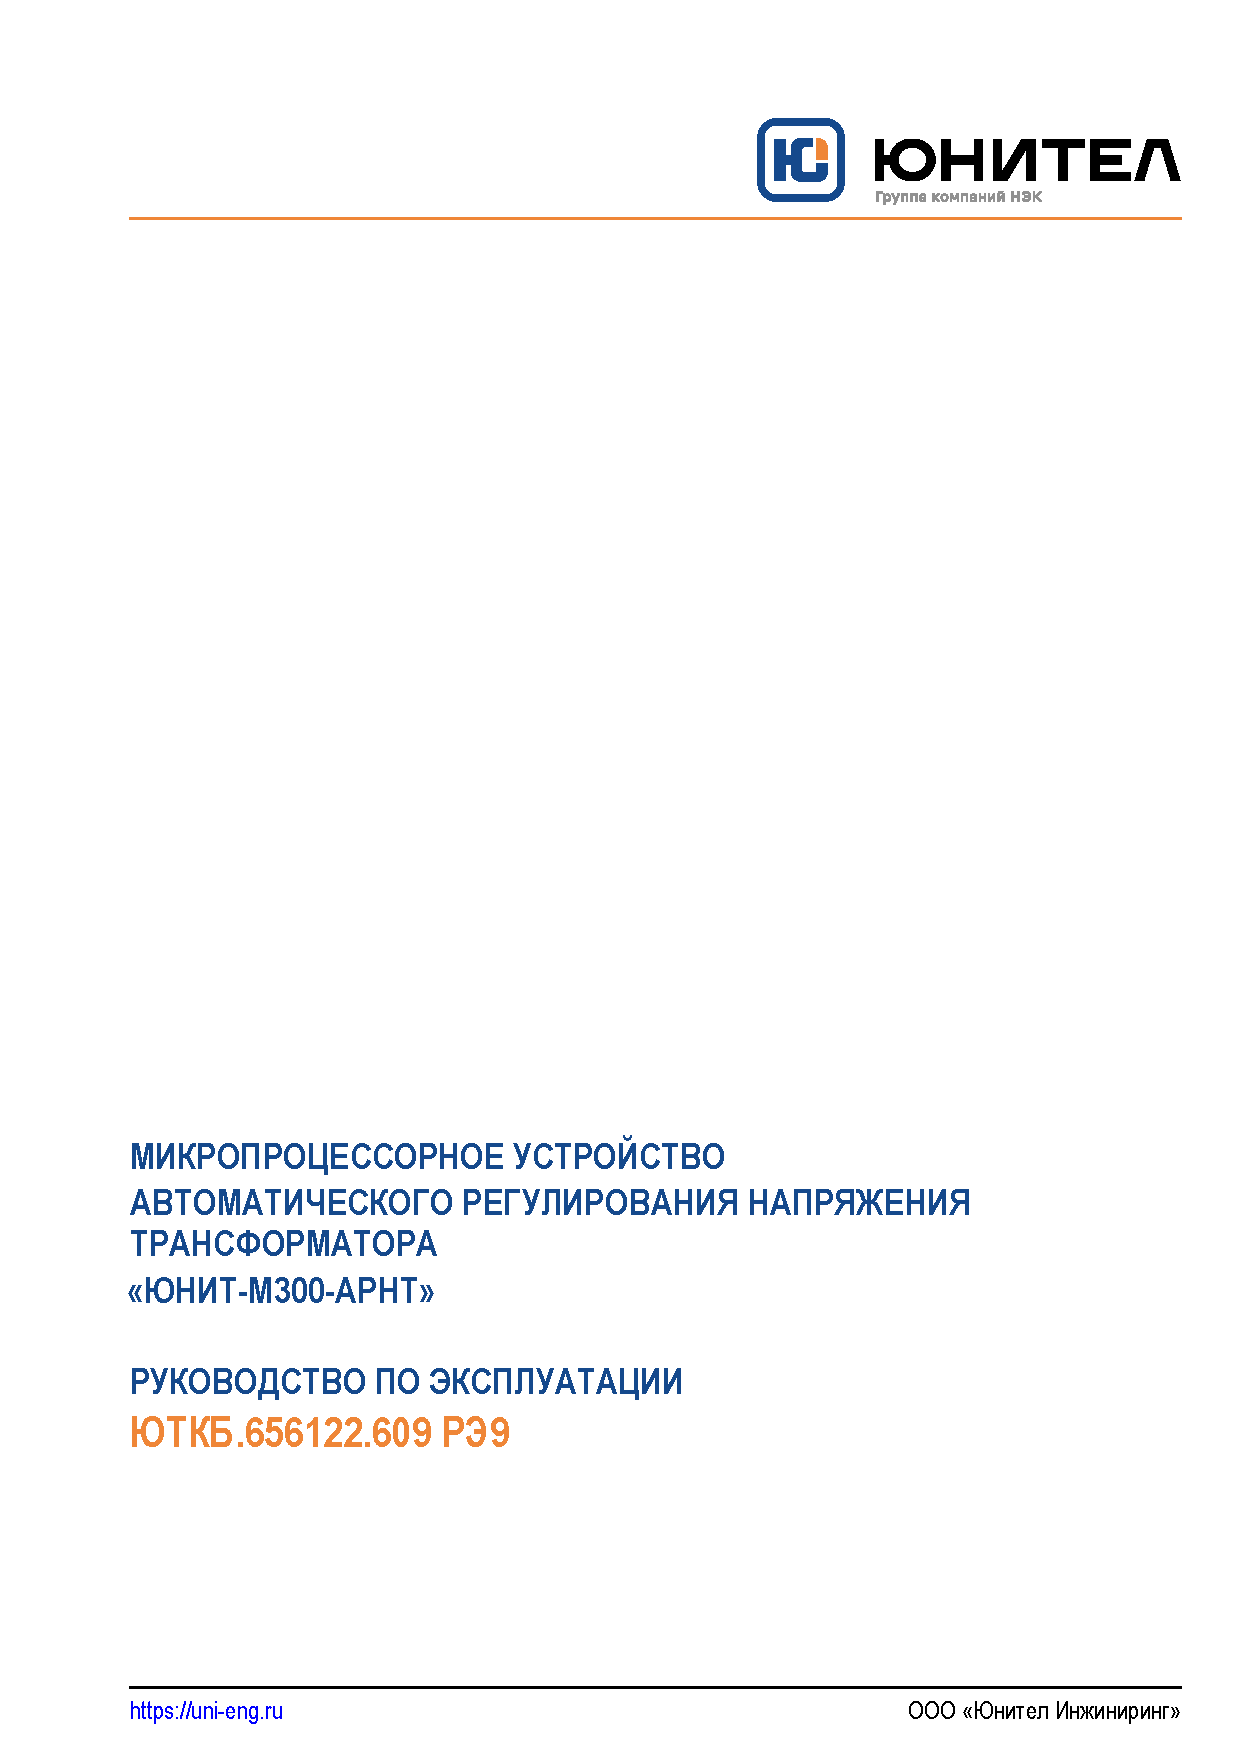
\includepdf[pages={1},width=0.5\textwidth, angle=90]{1.pdf} вставляем и поворачиваем pdf
%\begin{center}
%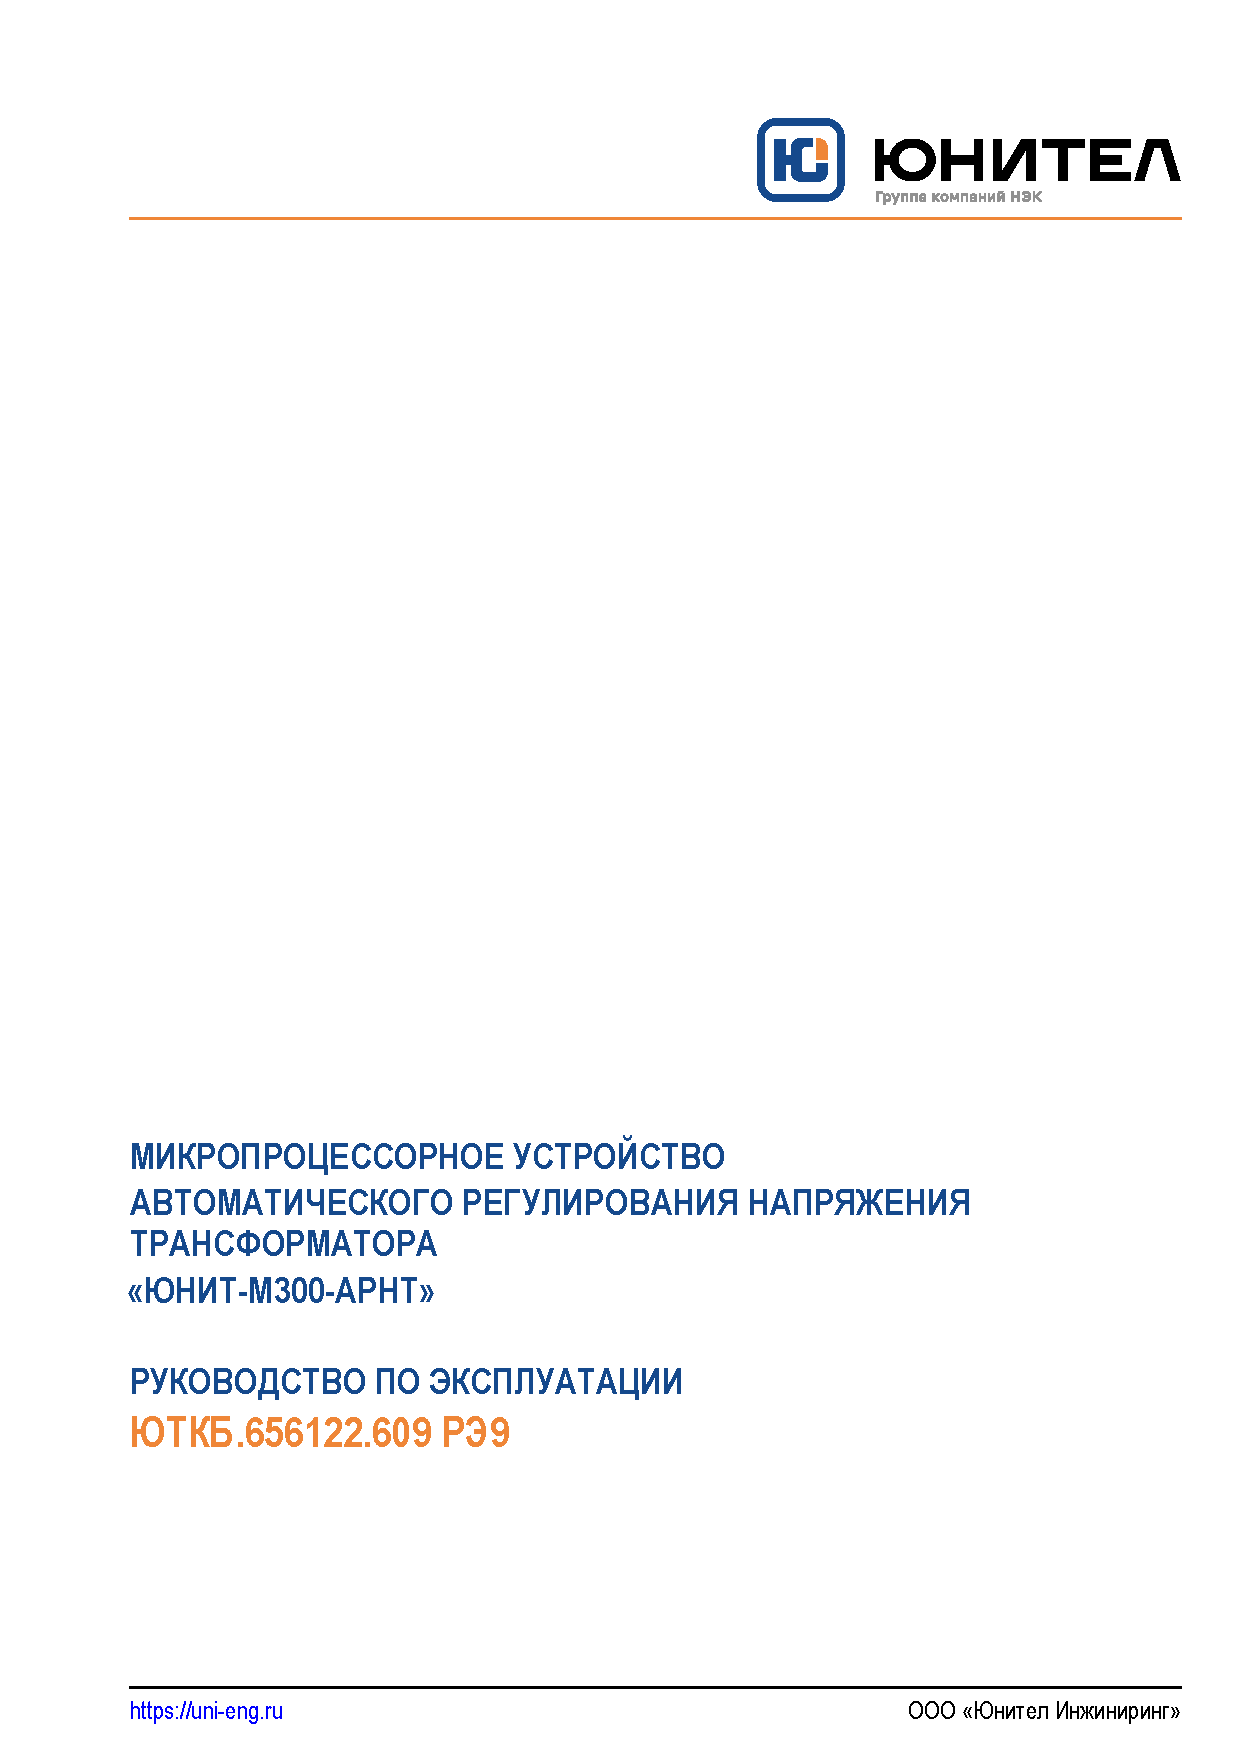
\includegraphics[width=1.4\textwidth]{1.pdf}
%\end{center}

\end{landscape}
\restoregeometry


